\apendice{Documentación técnica de programación}

\section{Introducción}
 En este apartado se describen los aspectos técnicos de programación.

\section{Estructura de directorios}
\begin{itemize}
    \item /: En este directorio se incluyen todos los documentos utilizados en el desarrollo del proyecto.
    \item /CNN y converter: En este directorio se incluyen los archivos Python con los que se ha obtenido la red neuronal convolucional y  el convertidor de keras a TensorFlow Lite.
    \item /CNN y converter/dataset: En este directorio se incluyen las fotos para entrenar la red neuronal convolucional.
    \item /app/retinopatia: En este directorio se encuentra el proyecto Android Studio. Incluyendo los archivos Gradle.
    \item /app/retinopatia/app: Directorio correspondiente a la aplicación.
    \item /app/retinopatia/app/src: Directorio donde se encuentra el código fuente.
    \item /app/retinopatia/app/src/androidTest: Directorio con los test de interfaz gráfica de la aplicación.
    \item /app/retinopatia/app/src/main: Directorio donde se encuentran los archivos principales de la aplicación.
    \item /app/retinopatia/app/src/main/assets: Directorio donde se almacenan recursos que se utilizan durante la ejecución de la aplicación.
    \item /app/retinopatia/app/src/main/java: Directorio donde se encuentran las clases creadas para la aplicación.
    \item /app/retinopatia/app/src/main/res: Directorio donde se encuentran más recursos, como son layouts, imágenes (drawables), strings, etc.
    \item /app/retinopatia/app/src/test: Directorio donde se encuentran los tests unitarios.
    \item /doc: Directorio que incluye el documento LaTeX.
\end{itemize}
\section{Manual del programador}
En esta sección se explicará lo que tiene que realizar futuros programadores para trabajar con la aplicación.

Al igual que en apartados anteriores, se va a separar el proyecto Android, del proyecto de Python de la red neuronal, para una mayor comprensión.

En el proyecto Android se necesita instalar los siguientes softwares:
\begin{itemize}
    \item Android Studio.
    \item Java JDK.
    \item SDK de Android.
    \item Emulador de Android.
\end{itemize}

Mientras que, para el proyecto de la red neuronal, se necesitan instalar:

\begin{itemize}
    \item Python 3.10.8.
    \item Un IDE, en mi caso Visual Studio Code, con la extensión de Python.
    \item NumPy
    \item Pandas
    \item matplotlib
    \item scikit-learn
    \item tensorflow
\end{itemize}

Además, es necesario la herramienta Git, para descargar el repositorio y navegar entre las distintas ramas, haciendo uso de un desarrollo continuo.

\textbf{Android Studio}

Android Studio es el IDE oficial de Android, diseñado por Google basandose en IntelliJ IDEA. Android Studio incluye la SDK de Android y Android Virtual Device, para la simulación de la aplicación. Ademas, con el soporte de Gradle se incluyen varios Java JDK para su utilización en el proyecto Android. 

En \ref{fig:Android Studio}, se puede observar la interfaz de Android Studio, y la emulación del dispositivo virtual creado con AVD, se pueden crear más AVD en \ref{fig:AVD}. Para la versión Android del dispositivo, se hace uso de la versión del SDK \ref{fig:SDK}, donde Android ofrece varios según la orientación del proyecto. Y por último, se puede ver en \ref{fig:JDK} como no es necesario la instalación de un JDK, puesto que lo incluye Gradle.

\begin{figure}[!ht]
         \centering
         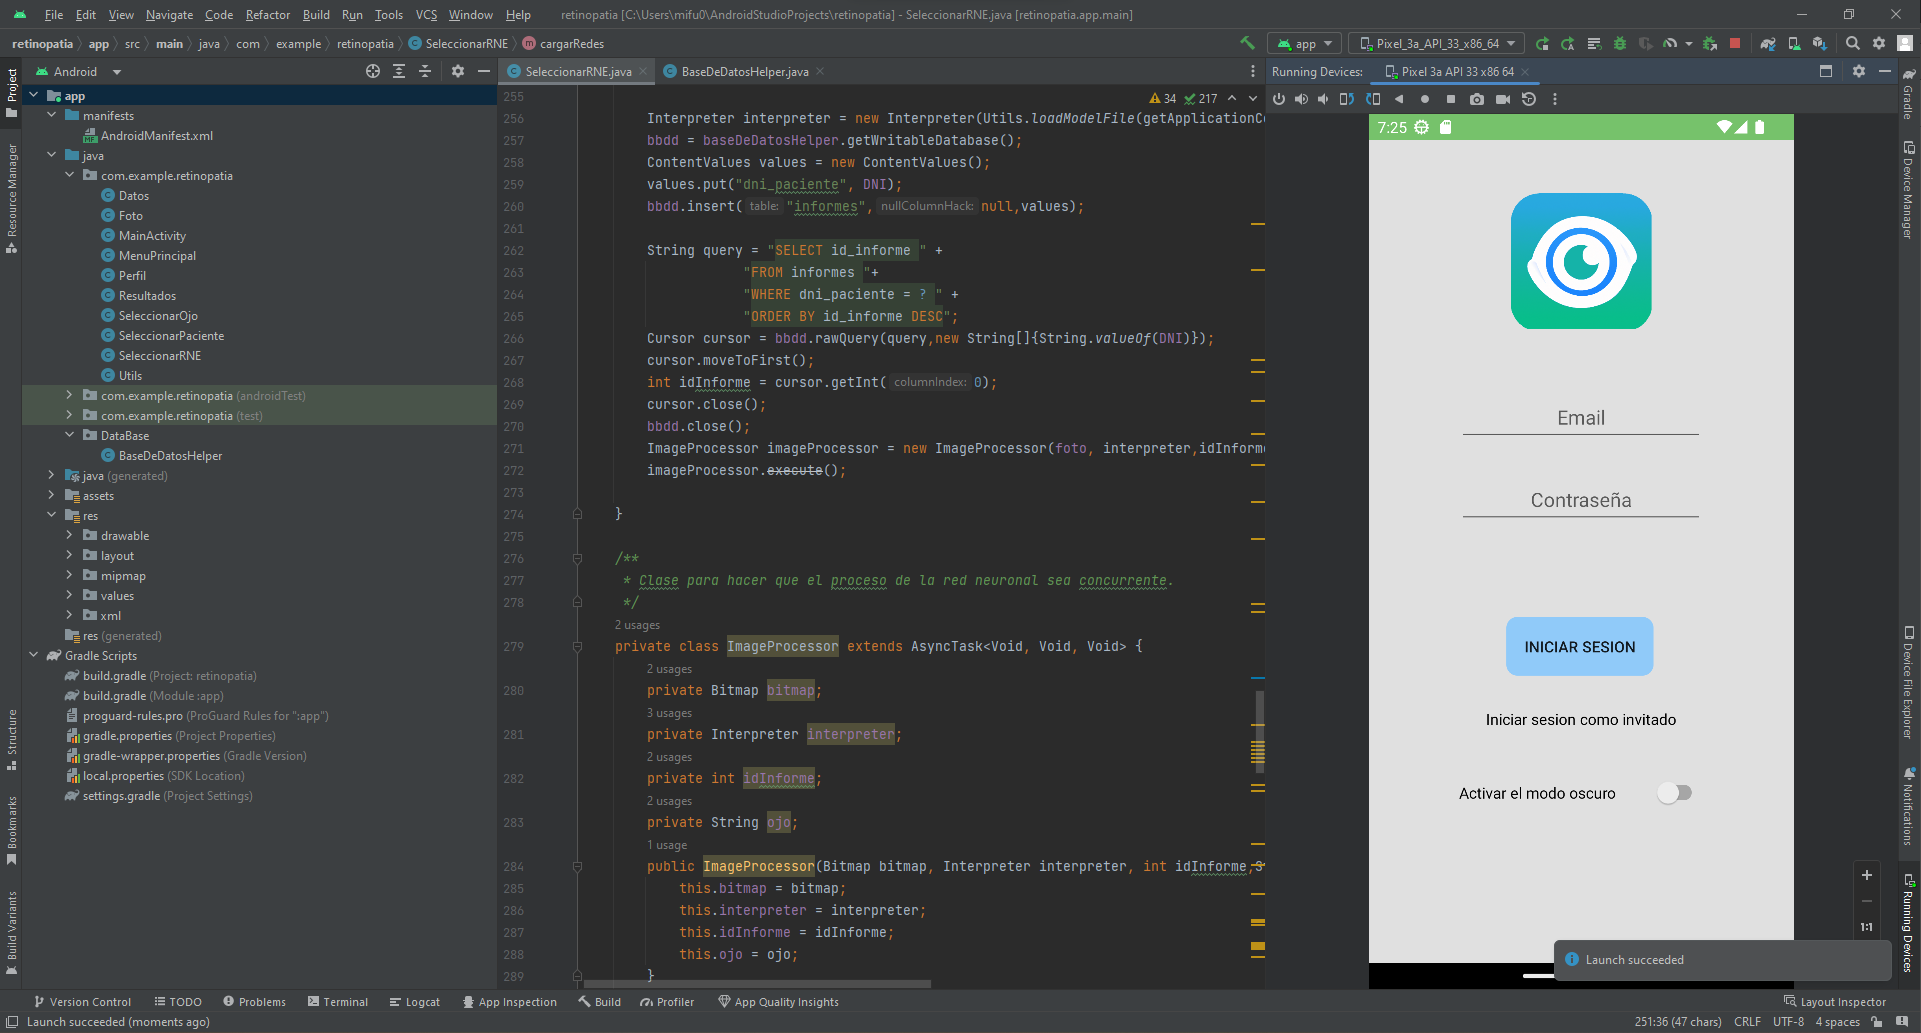
\includegraphics[width=0.9\textwidth]{img/Android Studio.png}
         \caption{Android Studio con un dispositivo virtual.}
         \label{fig:Android Studio}
\end{figure}
\begin{figure}[!ht]
         \centering
         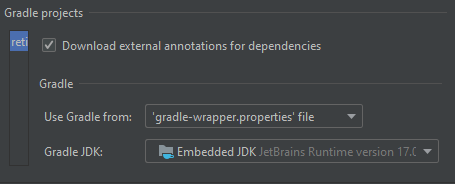
\includegraphics[width=0.9\textwidth]{img/JDK Graddle.png}
         \caption{Gradle incluye el JDK.}
         \label{fig:JDK}
\end{figure}
\begin{figure}[!ht]
         \centering
         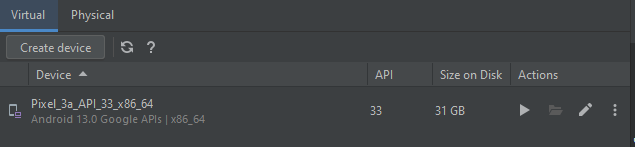
\includegraphics[width=0.9\textwidth]{img/AVD.png}
         \caption{Dispositivos virtuales Android.}
         \label{fig:AVD}
\end{figure}

\begin{figure}[!ht]
         \centering
         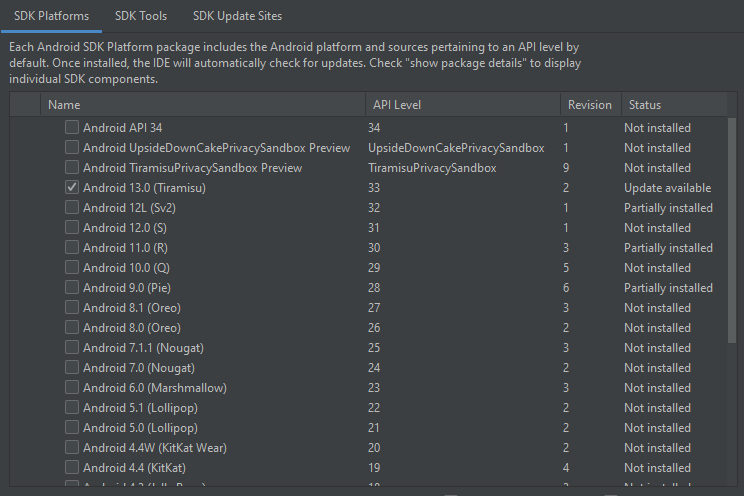
\includegraphics[width=0.9\textwidth]{img/SDK Android.png}
         \caption{SDKs ofrecidos.}
         \label{fig:SDK}
\end{figure}

\section{Compilación, instalación y ejecución del proyecto}

\subsection{Instalación}


Para instalar Android Studio, desde la página oficial se obtiene el ejecutable, puesto que es posible que el proyecto no sea compatible con futuras versiones de Android Studio, se ha utilizado la versión ``Flamingo 2022.2.1'', en caso de incompatibilidad, la página ofrece un aparatado para descargar \href{https://developer.android.com/studio/archive?hl=es-419}{versiones anteriores}.

Al descargar el ejecutable, se siguen las instrucciones, y el instalador instala automáticamente el SDK de Android y el emulador. Y el JDK se incluye en el Gradle del proyecto.

Para instalar Python, se descarga desde la página oficial, en este caso como ya es una versión anterior, se va al apartado de versiones anteriores y se descarga la versión 3.10.8.

Una vez instalado, se comprueba que la variable de entorno está configurada correctamente, en caso de no estarlo, el ``Path'' por defecto en Windows es: \textit{C:\textbackslash Users\textbackslash \$username\$\textbackslash AppData\textbackslash Local\textbackslash Programs\textbackslash Python\textbackslash Python310\textbackslash }. 

Para instalar las librerías de Python, se insertar 1 a 1 las siguientes líneas:

\lstdefinestyle{DOS}
{
    backgroundcolor=\color{black},
    basicstyle=\scriptsize\color{white}\ttfamily
}
\lstset{
  style=DOS,
  keywordstyle=\color{blue},
  commentstyle=\color{green!60!black},
  stringstyle=\color{red},
  showstringspaces=false,
  breaklines=true,
  breakatwhitespace=false,
  tabsize=4,
  numbers=none,
  numberstyle=\tiny,
  frame=single,
  framexleftmargin=5mm,
  xleftmargin=5mm
}
\begin{lstlisting}
cd C:\Users\$username$\AppData\Local\Programs\Python\Python310\Scripts\
pip install numpy
pip install pandas
pip install matplotlib
pip install scikit-learn
pip install tensorflow

\end{lstlisting}

Con las librerías instaladas, se procede a instalar el IDE, aunque también se puede usar un editor de texto y utilizar la consola para su ejecución. Como no es relevante el IDE que se utilice, no se comentará su instalación.

\subsection{Obtención del proyecto}

Para descargase el proyecto, se recomienda hacer uso de git. Para ello, se prepara el directorio donde se va a realizar el  proyecto, y posteriormente, se introduce el comando ``git clone https://github.com/mfg1014/Retinopatia-diabetica.git''.

Con el proyecto descargado, se pueden importar los archivos Python de la carpeta ``CNN y converter'' en el IDE que se use, en abrir carpeta. 

Para importar el proyecto Android, sería File > Open, y se selecciona la carpeta /app/retinopatía. Con ello, Android Studio detectará que es un proyecto Android, abriendo el proyecto para trabajar en él.

\subsection{Ejecución del proyecto}

Para el proyecto Python, la aplicación se ejecuta con el comando Python ``nombre del archivo''.py. Es importante tener en cuenta que el archivo de las redes neuronales tarda bastante, debido a que tiene que crear cada ejecución el modelo VGG-16, además, se crean 30 modelos, con sus respectivas matrices de confusión.

Para el proyecto Android se puede comprobar su ejecución de distintas formas:

\textbf{Emulador}

Android Studio ofrece un emulador incluido, donde se pueden probar las funcionalidades de la aplicación.

Para usar un emulador, se abre el Device manager, añadiendo un nuevo dispositivo, donde se selecciona entre varios dispositivos, en la realización de la práctica, se ha utilizado el dispositivo Pixel 3a con la versión Tiramisu, también se pueden seleccionar características como los núcleos de la CPU, la memoria RAM, el espacio del dispositivo,... Una vez creado, se abre el menú ``Run'', y se selecciona ``Run app''.

\textbf{Dispositivo físico}

Para usar un dispositivo físico es necesario habilitar las opciones de desarrollador, una vez hecho, se tiene que habilitar la opción de depuración ya sea por WIFI o por USB. Cuando se vincula con Android Studio, el dispositivo informa que se quiere añadir una aplicación mediante depuración, y una vez instalada se puede  usar como una aplicación normal.
\subsection{Errores encontrados y nuevas funcionalidades}

En caso de encontrar errores en la aplicación, se recomienda añadir una Issue al repositorio, donde se trabajará para solucionar el problema.

Si se quiere añadir nuevas funcionalidades, se recomienda crear una nueva rama por cada funcionalidad que se esté implementando concurrentemente.

\subsection{Crear una nueva realease}

Para crear una nueva release, es necesario obtener la apk para ello, en Android Studio, se hace lo siguiente:
\begin{itemize}
    \item Build > Build Bundle(s) /APK(s) > BUild APK(s).
    \item De esta forma, se genera el archivo .apk en el directorio ``app/build/outputs/apk/debug/''
\end{itemize}

Posteriormente, con el archivo APK, se comprime el directorio de la aplicación en un .zip y se va al repositorio al apartado releases, y se añade una nueva con estos archivos.

\section{Pruebas del sistema}

Como ya se ha comentado en el Diseño de pruebas, no se han realizado pruebas automáticas, pero cada vez que se realizaba un cambio de la aplicación, se comprobaba los casos de prueba relativos a las pruebas. Es importante aclarar que algunas funcionalidades no tienen pruebas específicas, pero de forma aleatoria se introducían en otros casos de prueba para comprobar el correcto funcionamiento.

Por otro lado, se han hecho pruebas en el emulador con una API Android 33 y en el dispositivo físico con una API Android 31. Por tanto, puede a ver errores en la visualización de los datos para versiones inferiores.

Mientras que en los archivos Python no es necesario el uso de pruebas.

Al finalizar el proyecto, todos los casos de prueba se pasaban correctamente.
